\chapter{Symulacja procesu}
	\label{ch:sym}
	
	\section{Charakterystyka statyczna}
	\label{sec:stat}
	
		Zadany układ opisany jest równaniami:
		\begin{equation}
		\left\{
		\begin{tabular}{l}
			$x_1(k)= - \alpha_1 x_1(k-1) + x_2(k-1) + \beta_1 g_1(u(k-3))$ \\\\
			$x_2(k)= - \alpha_2 x_1(k-1) + \beta_2 g_1(u(k-3))$\\\\
			$y(k)=g_2(x_1(k))$\\\\
		\end{tabular}
		\right.
		\label{eq:dyskretne}
		\end{equation}
		gdzie $u$-sygnał wejściowy, $y$-sygnał wyjściowy, $x_1$, $x_2$ - zmienne stanu, $\alpha_1 = -1,422574$, $\alpha_2 = 0,466776$, $\beta_1 = 0,017421$, $\beta_2 = 0,013521$ oraz
		\begin{equation}
			g_1(u(k-3))=\frac{exp(5u(k-3))-1}{exp(5u(k-3))+1},\quad g_2(x_1(k))=1-exp(-1.5x_1(k))
		\label{eq:g1g2}
		\end{equation}
		
		Podany punkt pracy układu to $u=y=x_1=x_2=0$, więc w wersji statycznej:
		\begin{equation}
			\left\{
			\begin{tabular}{l}
			$x_1= - \alpha_1 x_1+x_2+ \beta_1 g_1(u)$ \\\\
			$x_2= - \alpha_2 x_1+ \beta_2 g_1(u)$\\\\
			$y=g_2(x_1)$\\\\
			\end{tabular}
			\right.
			\label{eq:statyczne}
		\end{equation}
		
		Po przekształceniach:
		\begin{equation}
			x_1 = \frac{(\beta_1 + \beta_2)g_1(u)}{1+\alpha_1+\alpha_2}
			\label{eq:x1_static}
		\end{equation}
		
		Po podstawieniu równania (\ref{eq:x1_static}) do $y$ otrzymujemy
		\begin{equation}
			y(u) = g_2(\frac{(\beta_1 + \beta_2)g_1(u)}{1+\alpha_1+\alpha_2}
			\label{eq:y_static})
		\end{equation}
		
		Wykres wyznaczonej charakterystyki statycznej dla zadanego zakresu wartości sterowania ($u^{min}=-1, u^{max} = 1$) przedstawiony został na wykresie \ref{fig:stat}. Wykres został wygenerowany za pomocą skryptu $charakterystyka\_statyczna.m$.
		
		\begin{figure}[h!]
			\centering
			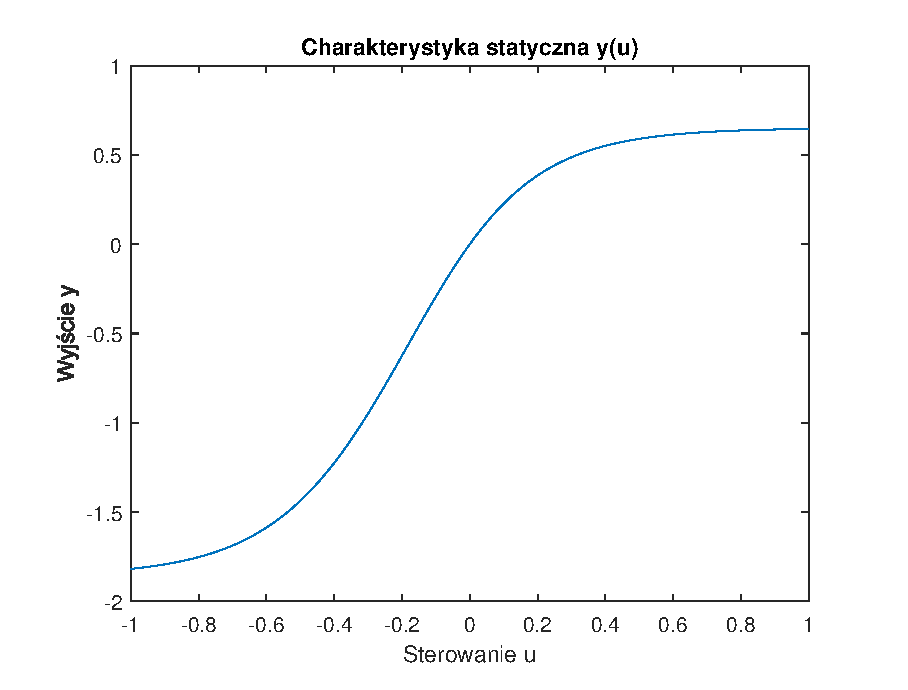
\includegraphics[width=\linewidth]{img/stat.eps}
			\caption{Charakterystyka statyczna procesu}
			\label{fig:stat}
		\end{figure}
		
	\section{Zbiory danych}
		\label{sec:dane}
		
		W celu przygotowania do uczenia sieci neuronowych wygenerowaliśmy dwa zbiory danych. Dane zostały wygenerowane poprzez zasymulowanie zadanego procesu dla sygnału sterowania złożonego o wartości zmieniającej się skokowo co 50 próbek. Obydwa zbiory danych mają po 2000 próbek. Zostały one przedstawione na wykresach \ref{fig:d_ucz} i \ref{fig:d_wer}. Użyte zostały skrypty: $generowanie\_danych.m$ (do wygenerowania danych) oraz $wykres\_dancyh.m$ (do narysowania wykresów).
		
		\begin{figure}[h!]
			\centering
			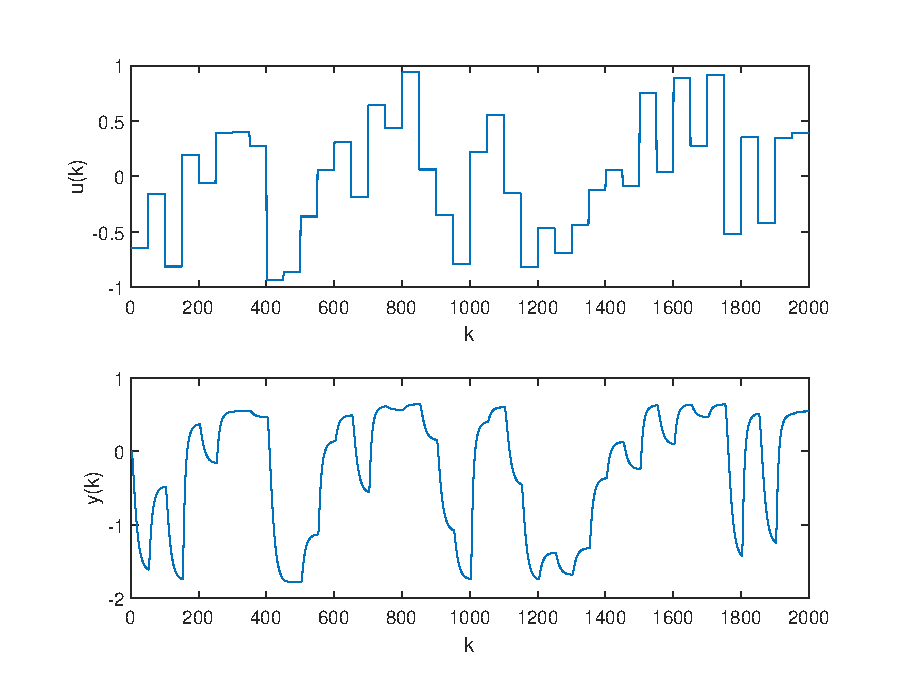
\includegraphics[width=0.9\linewidth]{img/dane_ucz.eps}
			\caption{Dane uczące}
			\label{fig:d_ucz}
		\end{figure}
		
		\begin{figure}[h!]
			\centering
			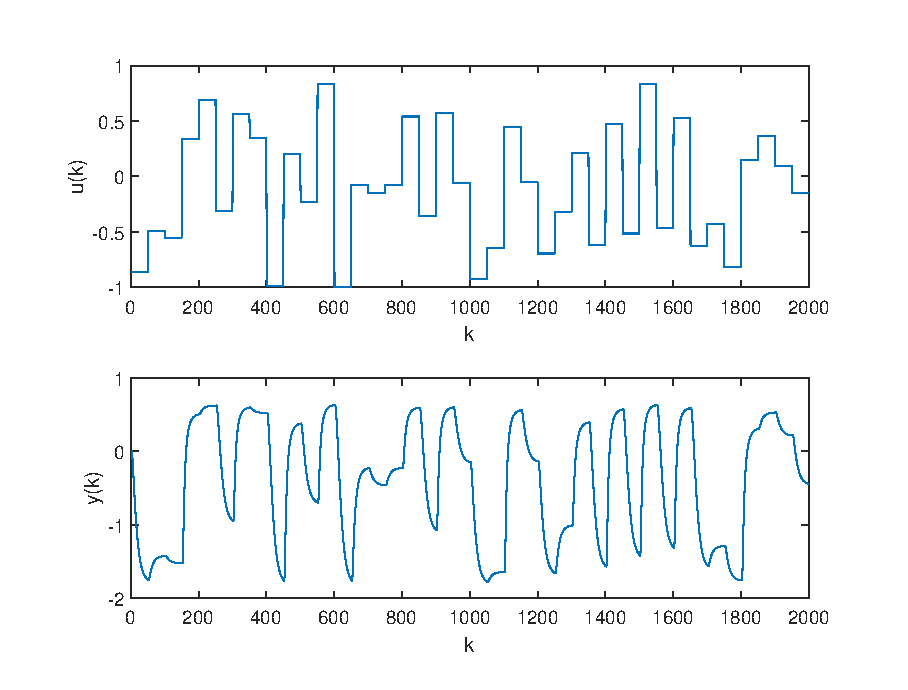
\includegraphics[width=0.9\linewidth]{img/dane_wer.eps}
			\caption{Dane weryfikujące}
			\label{fig:d_wer}
		\end{figure}